\documentclass{beamer}
\usepackage[utf8]{inputenc}
\usepackage{color}
\usepackage{ulem}
\usepackage{graphicx}
\usepackage[french]{babel}
\usepackage{hyperref}
\usepackage{multicol}
\hypersetup{pdfborder={0 0 0}, colorlinks=true, urlcolor=blue, linkcolor = darkred}
\selectlanguage{french}
\definecolor{darkred}{rgb}{0.85,0,0}
\definecolor{darkblue}{rgb}{0,0,0.7}
\definecolor{darkgreen}{rgb}{0,0.6,0}
\definecolor{darko}{rgb}{0.93,0.43,0}
\definecolor{maintitle}{rgb}{0.66,0,0.22}
\definecolor{title}{rgb}{0,0.5,0.5}
\definecolor{greyy}{rgb}{0.6,0.6,0.6}

\newcommand{\image}[1]{\includegraphics{#1}}
\newcommand{\imageR}[2]{\includegraphics[width=#2px]{#1}}
\newcommand{\imageRT}[2]{\includegraphics[height=#2px]{#1}}
\newcommand{\img}[1]{\begin{center}\includegraphics[width=400px]{#1}\end{center}}
\newcommand{\imag}[1]{\begin{center}\includegraphics{#1}\end{center}}
\newcommand{\imgR}[2]{\begin{center}\includegraphics[width=#2px]{#1}\end{center}}
\newcommand{\imgRT}[2]{\begin{center}\includegraphics[height=#2px]{#1}\end{center}}
\newcommand{\term}[1]{\textit{\textcolor{maintitle}{#1}}}
\newcommand{\cerm}[1]{\textcolor{maintitle}{#1}}
\newcommand{\gre}[1]{\textcolor{darkgreen}{#1}}
\newcommand{\blu}[1]{\textcolor{darkblue}{#1}}
\newcommand{\red}[1]{\textcolor{darkred}{#1}}

\usetheme{Warsaw}
\usecolortheme{beaver}
%\setbeamercolor{section in head/foot}{bg=black}
\setbeamercolor{title}{bg=maintitle,fg=white}

\title[The Mythical Man-Month $\sim$ Chapters 7 \& 8]{The Mythical Man-Month \\ $\sim$ \\ Chapter 7 : Why Did the Tower of Babel 
Fails ? \\ Chapter 8 : Calling the shot}
\author{Dubuc Xavier}

\institute{\imageR{UMONS.jpg}{100}}

\addtobeamertemplate{footline}{\insertframenumber/\inserttotalframenumber}

\begin{document}

\AtBeginSection[]
{
  \begin{frame}<beamer>
    \frametitle{Plan}
    \tableofcontents[currentsection,currentsubsection]
  \end{frame}
}

\AtBeginSubsection[]
{
  \begin{frame}<beamer>
    \frametitle{Plan}
    \tableofcontents[currentsection,currentsubsection]
  \end{frame}
}

\begin{frame}
\titlepage
\end{frame}

%%%%%%%%%%%%%%%%%%%%%%%%%%%%%%%%%%%%%%%%%%%%%%%% INTRODUCTION %%%%%%%%%%%%%%%%%%%%%%%%%%%%%%%%%%%%%%%%%

\section{Chapter 7 $\sim$ Why Did the Tower of Babel Fails ?}

\subsection*{Introduction et explication du titre}

\begin{frame}{Introduction}
Ce chapitre traite des essentiels que doit posséder un projet afin qu’il soit mené à son terme et ce, dans les meilleurs délais 
et avec la meilleure qualité. Les 2 eléments les plus importants à gérer dans un projet sont :
\pause
\begin{itemize}
\item \textbf{l'organisation}
\pause \item \textbf{la communication}
\end{itemize}
\end{frame}

\begin{frame}{Conséquence d'un manque de communication}
L'histoire nous apprend qu'un manque de communication peut être fatal à l'accomplissement d'un projet, c'est ce qui a eu lieu lors
de la construction de la tour de Babel.
\end{frame}

\begin{frame}{Exemple de la tour de Babel}
\begin{figure}
	\begin{center}
	\imageR{babel.jpg}{200}
	\caption{La tour de Babel}
	\end{center}	
\end{figure}
\end{frame}

\begin{frame}{Exemple de la tour de Babel : contexte}
Si on en croit la Génèse, le Seigneur, prenant peur de ce que pouvaient faire les hommes, est intervenu pour que la langue unique 
ne soit plus d'actualité et ainsi compromettre la \red{communication} entre les hommes ce qui a mené à un manque 
d'\red{organisation}.

\begin{figure}
	\begin{center}
	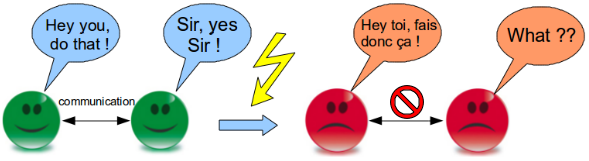
\includegraphics[width=225px]{img_001.png}
	\caption{Problème de communication dû à la langue}
	\end{center}	
\end{figure}
\end{frame}

\begin{frame}{Exemple de la tour de Babel : enseignements}
Le manque de \red{communication} mène à :
\begin{itemize}
\pause \item des disputes,
\pause \item de la jalousie,
\pause \item une isolation des gens (ils évitent les querelles)
\end{itemize}
\pause En conséquence, l'\red{organisation} s'en trouve affectée car ils ne peuvent se coordiner ce qui a eu pour effet, dans le 
cas de la tour de Babel, de stopper le projet.
\end{frame}

\subsection{La communication dans les grands projets de programmation}

\begin{frame}{Introduction}
De nos jours, 
\begin{itemize}
\item les problèmes de calendrier,
\item les incompatibilités fonctionnelles,
\item les bugs de système,
\end{itemize}
surgissent à cause du fait qu'une partie du projet ne sait pas ce que font les autres parties.

\begin{exampleblock}{Exemple}
La partie s'occupant de la gestion des coûts ne sait pas forcément ce que fait la partie s'occupant de la production.
\end{exampleblock}
\end{frame}

\begin{frame}
Pour éviter tous ces désagréments, les différentes parties d'un projet doivent avoir une \gre{bonne communication} et ce, de 
toutes les manières possibles :
\begin{itemize}
\pause \item \textbf{\red{de manière informelle}} : \textit{via un bon service téléphonique et une définition claire des 
dépendances entre groupes,}
\pause \item \textbf{\red{via des réunions}} : (précieuses) \textit{réunions de projet régulières où les différentes équipes 
présentent des briefings techniques,}
\pause \item \textit{un utilisant un \textbf{\red{''Project Workbook"}}} (littéralement ''classeur de projet") \textit{que l'on 
initialise dès le début du projet.}
\end{itemize}
\end{frame}

\subsection{Le ''Project Workbook"}

\begin{frame}{Project Workbook : Définition}
Ce \textit{project workbook (\textbf{PW})}, est un document à part régissant la structure des documents que le projet va fournir
quoi qu'il arrive. Chacun de ces documents doit faire partie de cette structure, cela inclut :
\begin{itemize}
\pause \item les objectifs,
\pause \item les spécifications externes,
\pause \item les spécifications internes,
\pause \item les spécifications de l'interface,
\pause \item les standards techniques,
\pause \item les mémos administratifs.
\end{itemize}
\end{frame}

\begin{frame}{Project Workbook : Utilités}
\begin{enumerate}
\item Si on examine la généalogie d'un tel document, on peut non seulement \textbf{retracer les idées} mais aussi une grande 
partie des phrases du premier mémo qui propose le produit ou explique le premier design.
\pause\item Il permet le \textbf{contrôle de la distribution de l'information}. L'idée n'est pas de restreindre l'information mais 
d'assurer que l'information pertinante parvienne à toutes les personnes qui en ont besoin.
\end{enumerate}
\end{frame}

\begin{frame}{Project Workbook : En pratique}

Le problème du \textbf{PW} n'est \red{pas linéaire} avec la taille du projet, ainsi, plus le projet rassemble de gens, plus le 
\textbf{PW} est grand (en taille) et plus il est \textbf{nécessaire} pour la bonne organisation du projet.\\
$ $\\
$\Rightarrow$ \textbf{Importance de trouver un \underline{bon} moyen de le tenir à jour.}

\end{frame}

\begin{frame}{Project Workbook : Cas de l'OS/360}

Ils disposaient d'un système d'édition de texte dirigé par un ordinateur pour éditer un \textbf{PW} à feuilles mobiles (ils 
imprimaient les modifications). 
\begin{itemize}
\pause \item au début du projet, ils en étaient totalement contents,
\pause \item après \textbf{6 mois} consacrés au projet, les premiers problèmes sont apparus, problèmes liés à la \red{taille du 
\textbf{PW}} :
\begin{itemize}
\pause \item une copie de ce \textbf{PW} faisait \red{1,524m de large}, les \red{mises à jour 5cm} \textit{(environ 150 pages)}
\pause \item possédant 100 bureaux, il y avait donc 100 copies de ce \textbf{PW}, en les empilant, la pile dépassait le toit du
\textit{Manhattan's Time-Life Building}.
\end{itemize}
$\Rightarrow$ \red{l'entretien du \textbf{PW} prenait un temps conséquent !}
\end{itemize}

\end{frame}

\begin{frame}{Project Workbook : Cas de l'OS/360}

\begin{figure}
	\begin{center}
	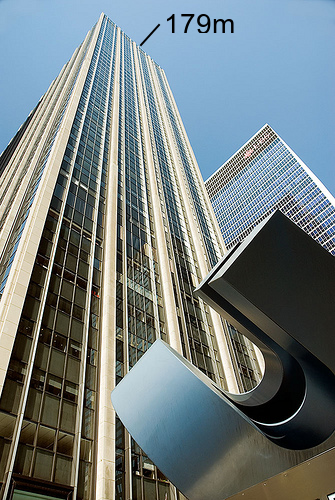
\includegraphics[width=100px]{img1.png}
	\caption{Manhattan's Time-Life Building}
	\end{center}	
\end{figure}

\end{frame}

\begin{frame}{Project Workbook : Cas de l'OS/360 $\sim$ Solution}
Solution employée : passage aux \textbf{microfiches}, 
\begin{itemize}
\item[$\Rightarrow$] 1 million de dollars sauvés,
\item[$\Rightarrow$] le \textbf{PW} a diminué de $0.0849 m^3$ à $0.00429 m^3$ \textit{(division par 2 du volume !)} et les 
mises à jour apparaissaient par morceau de centaines de pages, réduisant par 100 le problème d'insertion.\\
\end{itemize}
Néanmoins, ces microfiches ont leurs \red{inconvénients}, elles ne peuvent pas, par exemple, être marquées, surlignées, ... il est 
donc moins évident de se rendre compte des modifications apportées à un document. \\

\end{frame}

\begin{frame}{Project Workbook : Les années 90}

Avec la technologie de systèmes qui arrivent, la meilleure technique, selon le livre, est de garder le \textbf{PW} sur des 
fichiers à accès direct, marqué par des barres de changements et des dates de révision. 
\begin{itemize}
\item Chaque utilisateur le consultait depuis un terminal d'affichage \textit{(les machines à écrire sont trop lentes)},
\item un résumé des changements, préparé chaque jour, serait stocké de manière \textbf{LIFO} dans un point d'accès fixé,
\end{itemize}

\end{frame}

\begin{frame}{Project Workbook : Les années 90}

Les \gre{avantages} sont notables, par exemple :
\begin{itemize}
\item un programmeur devrait normalement lire ces résumés chaque jour, mais admettons 
qu'il soit malade 2-3 jours, à son retour il n'aurait qu'à lire ces résumés pour se tenir au courant des changements qui ont eu 
lieu en son absence.
\item \textbf{de plus}, il peut s'interrompre pendant sa lecture pour consulter le texte dans le \textbf{PW} qui 
est concerné par les modifications reprises dans le résumé.
\end{itemize}

\end{frame}

\subsection{L'organisation dans les grands projets de programmation}

\begin{frame}{Introduction}
$n$ travailleurs dans un projet 
\begin{itemize}
\item[$\Rightarrow$] $\dfrac{n^2-n}{2}$ interfaces de communication différentes,
\item[$\Rightarrow$] $2^n$ équipes potentielles à coordonner. \\
\end{itemize}
$ $\\
Le but de l'\textbf{\red{organisation}} est de réduire le nombre de \textbf{communications} et de \textbf{coordinations} 
nécéssaires.
\end{frame}

\begin{frame}{Éviter les communications}
Pour \textbf{éviter les communications}, il est recommandé d'appliquer les principes élémentaires de \textbf{management} tels que 
\href{http://blogconsultantfrance.blogspot.com/2008/08/les-14-principes-du-management-de-henri.html}{les principes de 
\textbf{Fayol}}. Les plus importants en ce qui nous concerne sont : 
\begin{enumerate}
\item la division du travail,
\item la spécialisation fonctionnelle.
\end{enumerate}
Ces 2 principes impliquent que la structure de l'entreprise tende vers un arbre, afin de respecter un autre de 
\href{http://blogconsultantfrance.blogspot.com/2008/08/les-14-principes-du-management-de-henri.html}{ces principes de 
\textbf{Fayol}}, l'\textbf{unicité du supérieur hiérarchique direct}.
\end{frame}

\begin{frame}{Unicité du chef : pourquoi ?}
\begin{figure}
	\begin{center}
	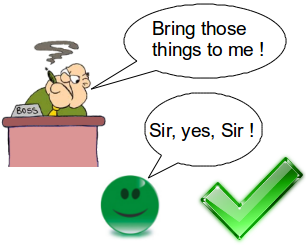
\includegraphics[width=100px]{img_002.png}
	\caption{Principe du chef unique respecté.}
	\end{center}	
\end{figure}
\end{frame}

\begin{frame}{Unicité du chef : pourquoi ?}
\begin{figure}
	\begin{center}
	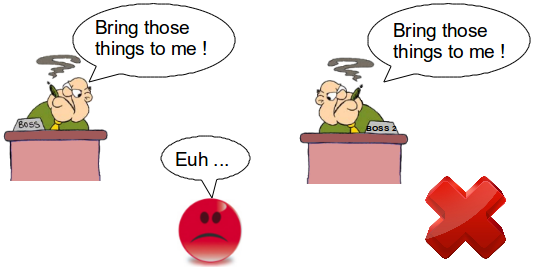
\includegraphics[width=200px]{img_003.png}
	\caption{Principe du chef unique non-respecté.}
	\end{center}	
\end{figure}
\end{frame}

\begin{frame}{Structure}
Chaque sous-arbre de la structure se doit de contenir les éléments suivants pour être fonctionnel :
\begin{enumerate}
\pause \item une mission,
\pause \item \red{un producteur},
\pause \item \red{un directeur technique},
\pause \item un calendrier,
\pause \item \textbf{une division du travail},
\pause \item des définitions d'interfaces entre les parties.
\end{enumerate}
Toutes ces choses sont conventionnelles et évidentes, mis à part la distinction entre le \red{producteur} et le \red{directeur 
technique}.
\end{frame}

\begin{frame}{Rôles du producteur}
\begin{itemize}
\item Rassembler l'équipe
\pause \item Diviser le travail
\pause \item Établir le calendrier et s'assurer qu'il est respecté
\pause \item Acquérir les ressources nécessaires
\pause \item Établir le modèle de communication et de rapports à l'intérieur de l'équipe
\end{itemize}
\pause Cela signifie qu'une majeure partie de son rôle consiste en \textbf{communications en dehors de son équipe} 
\textit{(envers les instances supérieures ou avec des collègues du même niveau que lui)}.
\end{frame}

\begin{frame}{Rôles du directeur technique}
\begin{itemize}
\item Concevoir le design
\pause\item Identifier les sous-parties
\pause\item Spécifier à quoi le projet va ressembler vu de l'extérieur
\pause\item Esquisser la structure interne
\pause\item Fournir l'unité et l'intégrité conceptuelle à tout le design
\pause\item Servir de limite à la complexité du système
\pause\item Inventer des solutions à d'éventuels problèmes techniques qui surgissent (ou changer le design en conséquence)
\end{itemize}
\pause Ses \textbf{communications sont principalement "intra-équipe"} et son travail est presque entièrement technique.\\
\end{frame}

\begin{frame}{Relation producteur-directeur technique}
Après avoir bien différencier ces 2 fonctions, il est clair que les 2 rôles demandent des talents différents, il y a dès lors 3
situation possibles :
\pause \begin{enumerate}
\item le producteur et le directeur technique sont une seule et même personne,
\item le producteur est le boss et le directeur technique son bras droit,
\item le directeur technique est le boss et le producteur son bras droit,
\end{enumerate}
\end{frame}

\begin{frame}{Le producteur et le directeur technique sont une seule et même personne}
Cette situation est réalisable sur de \textbf{très petites équipes} \textit{(typiquement de 3 à 6 programmeurs)} mais au delà, 2 
problèmes se posent :
\begin{enumerate}
\pause \item la personne la meilleure en \textbf{management} et en \textbf{technique} est rarement trouvée,
\pause \item il est \textbf{difficile} pour le producteur de déléguer assez de ses fonctions pour s'occuper de son rôle de 
directeur technique et, dans l'autre sens, c'est \textbf{impossible} pour le directeur technique de déléguer sans compromettre 
l'intégrité conceptuelle du projet.
\end{enumerate}
\end{frame}

\begin{frame}{Le producteur est le boss et le directeur technique son bras droit}
\begin{itemize}
\item Difficulté d'établir l'autorité du directeur technique à prendre des décisions sans impact tel sur son temps qu'il serait 
placé dans la chaine de commande du management.
\item Les 2 hommes doivent avoir la même vue sur la philosophie technique fondamentale.
\item Ils doivent discuter sur les questions techniques de manière privée avant qu'elles ne deviennent opportunes.
\end{itemize}
\textbf{Cette structure peut être organisée pour être efficiente mais est, hélas, rarement essayée en pratique.}
\end{frame}

\begin{frame}{Le directeur technique est le boss et le producteur son bras droit}
Le producteur se doit de proclamer l'autorité suprême du directeur technique tout en restant ultra disponible et au petit soin 
pour lui de manière à ce que ce dernier n'ait à s'occuper que de l'ingénierie.\\
$ $ \\
\textbf{Cet arrangement peut également être organisé de manière à fonctionner de manière effective, mais \blu{Brooks} suspecte que 
cet arrangement est mieux adapté pour les petites équipes.}
\end{frame}

\begin{frame}{Structure idéale}
Selon \blu{Brooks}, la structure dans laquelle le \textbf{directeur technique} est le boss est la plus fiable pour les plus gros 
sous-arbres d'un projet vraiment gros.
\begin{figure}
    \begin{center}
    
\includegraphics[width=125px]{img_004.png}
    \caption{Structure idéale}
    \end{center}	
\end{figure}
\end{frame}

\subsection*{Conclusion}

\begin{frame}{Conclusion du chapitre}
\begin{itemize}
\item \textbf{La tour de Babel} était peut-être le premier fiasco de l'ingénieurie mais ce n'était clairement \textbf{pas le 
dernier}.
\item La \textbf{communication} et ses conséquences ainsi que l'\textbf{organisation} sont \red{critiques} pour la réussite d'un 
projet.
\item Les \textit{techniques de communication} et d'\textit{organisation} demandent du manager \textbf{plus de pensées} et 
\textbf{autant de compétences d'expérience que la technologie du logiciel lui-même}.
\end{itemize}
\end{frame}

%% NOW : FORGES ?

\section{Chapter 8 $\sim$ Calling the shot}

\subsection*{Introduction}

\begin{frame}{Entrée en matière}
\begin{center}
\begin{multicols}{2}
	
\includegraphics[width=50px]{publilius.jpg} \\
	\textit{"La pratique est le meilleur des instructeurs"} \\
	$ $ \\
	\textbf{Publilius Syrus.} (poête latin) \\
\end{multicols}
\end{center}
$ $ \\
\begin{center}
\begin{multicols}{2}
\textit{"L'expérience est cher enseignant, mais les fous n'apprendront à personne."} \\
$ $ \\
\textbf{Benjamin Franklin.} \\
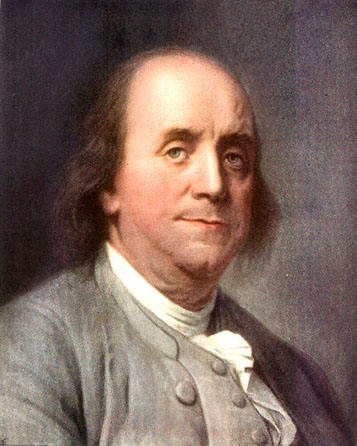
\includegraphics[width=50px]{franklin.jpg}\\
\end{multicols}
\end{center}

\end{frame}

\begin{frame}{Fil directeur}

Comment peut-on estimer 
\begin{itemize}
\pause \item le \red{temps} que va prendre un projet ?
\pause \item les \red{efforts nécessaires} à sa réussite ? \pause \\
\end{itemize}
$ $\\
Cette partie se base sur des \textbf{résultats expérimentaux} publiés par différents managers de projet afin de répondre au mieux 
à ces questions.
\end{frame}

\begin{frame}{Préambule}
Il faut savoir qu'il \textbf{ne suffit pas d'estimer la portion de code} mais qu'il faut également tenir compte : 
\begin{itemize} \pause
\item du planning,
\item de la documentation,
\item des tests (des composants et du système),
\item de l'intégration du système
\item des temps de formation.
\end{itemize}
\end{frame}

\begin{frame}{Préambule}
Il faut également considérer le fait que les données trouvées sur un \textbf{petit projet} ne seront pas forcément applicables aux 
\textbf{grands projets}, et inversément. \\
$ $\\
Des études ont montré que l'effort à fournir augmente comme une puissance de la taille du projet et qu'il pouvait être estimer 
comme suit : \begin{center}\red{effort} $=$ (constante) $\times (\text{\blu{nombre d'instructions}})^{1.5}$\end{center}

\end{frame}

\begin{frame}{Introduction aux données}
Cette partie présente à présent différentes données recueillies par des managers lors de leurs expériences professionnelles, ces 
données concernent toutes la \textbf{productivité} d'un programmeur.
\end{frame}

\subsection{Les données de Portman}

\begin{frame}{Portman}
\textbf{Charles Portman}, \textit{manager de ICL's Software Division, Computer Equipment Organization (Northwest) à Manchester} ; 
a découvert que \textbf{seulement la moitié} du temps que possède un programmeur est employé pour programmer et debugger. \\
$ $\\
Le reste du temps est occupé par:
\begin{itemize}
\item des \red{réunions},
\item de la \red{paperasse},
\item des éventuelles \red{maladies},
\item ...
\end{itemize}
\end{frame}

\begin{frame}{Portman}
$\Rightarrow$ Les estimations font une \textbf{hypothèse irréaliste} à propos du nombre d'heures de technique par personne/an.
\end{frame}

\subsection{Les données de Aron}
\begin{frame}{Aron}
\textbf{Joel Aron}, \textit{manager de Systems Technology chez IBM à Gaithersburg dans le Maryland}, a étudie la productivité d'un 
programmeur lorsqu'il travaille sur \underline{9 grands projets}.\\
\textit{(grand = plus de 25 programmeurs et plus de 30 000 instructions livrables)}\\
$ $\\
Il en a dégagé la loi suivante : \\
\begin{center}Nombre d'interactions entre programmeurs $\nearrow$ \\ $\Rightarrow$ \red{Productivité $\searrow$}\end{center}
\end{frame}

\subsection{Les données de Harr}

\begin{frame}{Harr}
\textbf{John Harr}, \textit{manager de programmation pour Bell Telephone Laboratories' Electronic Switching System} a réuni des 
données concernant \textbf{4 programmes de taille similaire} différents uniquement au niveau :
\begin{itemize}
\item de la taille des groupes de travail,
\item du temps pris,
\item du nombre de modules.
\end{itemize}
$\Rightarrow$ On constate dès lors que ces programmes donnent des productivités complètement différentes, celà étant probablement 
dû à la complexité des problèmes mais on ne peut que faire des suppositions. 
\end{frame}

\subsection{Les données de l'OS/360}
\begin{frame}{OS/360}
Ces données confirment la conclusion précédente, c'est-à-dire que la productivité est fortement liée à la complexité et à la 
difficulté de la tâche à effectuer.
\end{frame}

\subsection{Les données de Corbató}

\begin{frame}{Corbató}
\textbf{Corbató} du \textit{MIT's Project MAC} a recueilli des données sur le système d'exploitation MULTICS (entre 1 million et 2 
millions de mots dans le langage de programmation PL/1 (ancêtre du REXX)), ces données suggèrent 2 conclusions importantes :
\begin{enumerate}
\item La productivité semble être constante en terme de statement élémentaire (mots/lignes de code),
\item La productivité peut être \gre{\textbf{multipliée par 5}} lorsqu'un langage de programmation de haut niveau approprié est 
utilisé !
\end{enumerate}
\textit{(Les données précédentes concernaient toutes la programmation en langage assembleur)}
\end{frame}

\subsection*{Conclusion}
\begin{frame}{Conclusion}
\begin{enumerate}
\item Il faut \textbf{estimer de manière prudente} le temps pris par un programmeur pour finir son travail, ce temps devant 
comprendre les réunions, les éventuelles maladies, ...
\pause\item La productivité (et donc l'effort fourni et le temps pris pour le fournir) du programmeur dépend fortement de la 
\textbf{complexité et de la difficulté du problême} qui lui est 
soumis.
\pause\item L'utilisation d'un langage de programmation de haut niveau \textbf{multiplie par 5} la productivité.
\end{enumerate}
\end{frame}

\section{Analyse et critique}

\begin{frame}{Points forts}
\begin{itemize}
\item Mise en avant l'importance du management.
\item Structure irréprochable.
\item Approfondissement de chaque terme utilisé.
\end{itemize}
\end{frame}

\begin{frame}{Points faibles}
\begin{itemize}
\item Anglais assez soutenu.
\item Résultats concernant d'anciens projets, pas très représentatifs à nos yeux.
\item Utilisation de la théorie en pratique pas d'actualité (microfiches, terminaux d'affichage, ...).
\item Utilisation de la première personne pour la narration (\sout{objectivité}).
\end{itemize}
\end{frame}

\begin{frame}{Apprentissage}
Peu de choses non connues, en effet, la plupart du temps l'auteur parle de principes qui sont la base du management. Ces mêmes 
principes que nous avons vu dans le cours du même nom l'année passée. \\
$ $\\
Le livre n'étant pas très récent, il parle à peine des techniques disponibles de nos jours pour gérer un \textbf{Project Workbook} 
de manière simple.
\end{frame}

\begin{frame}{Project Workbook de nos jours}
Il existe de nombreuses solutions informatiques,
\begin{itemize}
\item pour les projets open-source, les \href{http://fr.wikipedia.org/wiki/Forge_(informatique)}{forges} sont recommandées,
\item pour les autres projets, il existe des logiciels tels que \href{http://www.microsoft.com/france/office/project/}{Microsoft 
Project} qui permettent de gérer un projet de A à Z de manière simple.
\end{itemize}
\end{frame}

\section{Bibliographie}

\begin{frame}{Bibliographie}
\begin{itemize}
\item[\red{\textbullet}] \red{Brooks, F.P} : \textit{The Mythical Man-Month : Essays on Software Engineering. 20th anniversary 
edn. Addison-Wesley (1995)}
\item[\red{\textbullet}] \red{Forge} : \textit{http://fr.wikipedia.org/wiki/Forge\_(informatique)}
\item[\red{\textbullet}] \red{Microsoft Project} : \textit{http://www.microsoft.com/france/office/project/}
\end{itemize}
\end{frame}
\end{document}